\documentclass[sigconf,nonacm]{acmart}

\usepackage{booktabs}
\usepackage{tabularx}
\usepackage{tikz}
\usetikzlibrary{arrows.meta,positioning,fit,backgrounds}

\newcolumntype{L}{>{\raggedright\arraybackslash}X}
\settopmatter{printfolios=true}

\begin{document}

\title{Antfly: An Inference-Native Polymorphic Database}

\author{AJ Roetker}
\authornote{Corresponding author.}
\email{aj@antfly.io}
\affiliation{%
  \institution{Antfly, Inc.}
  \city{Portland}
  \state{Oregon}
  \country{USA}}

\author{Rowan Copley}
\email{rowan@antfly.io}
\affiliation{%
  \institution{Antfly, Inc.}
  \city{Portland}
  \state{Oregon}
  \country{USA}}

\author{Tim Kaye}
\email{tim@antfly.io}
\affiliation{%
  \institution{Antfly, Inc.}
  \city{Portland}
  \state{Oregon}
  \country{USA}}

\author{Drew Lanenga}
\email{drew@antfly.io}
\affiliation{%
  \institution{Antfly, Inc.}
  \city{Portland}
  \state{Oregon}
  \country{USA}}

\renewcommand{\shortauthors}{Roetker et al.}

\begin{abstract}
Before data can be queried, applications derive representations of it with
models: transcripts, extracted text, chunks, embeddings, entities and
redactions. These are produced by external pipelines and stored as ordinary
records. The database cannot tell whether they are current, mutually
compatible, authorized or complete. Building and operating these pipelines is
inference engineering, and we argue its correctness contract belongs in the
database.

We present Antfly, an open-source (Apache-2.0) inference-native polymorphic
database that treats inference-derived artifacts as database-managed state.
Each artifact is bound to its source version, producer configuration and
model revision. A durable producer graph provides replay, dependency tracking
and explicit readiness. Documents, text, vectors, graph relationships and
relational data share one canonical identity, so filters and authorization
rules compose inside retrieval rather than through application-side joins.

We describe the architecture, its consistency and failure semantics, and the
costs of owning derived state while keeping inference compute disaggregated.
We propose experiments that test these guarantees against a well-built
external pipeline, including where ownership costs more.
\end{abstract}

\maketitle

%--------------------------------------------------------------------------
\section{Introduction}

Each wave of applications has brought a new kind of index, with consistency
trade-offs to match:

\begin{itemize}
  \item \textbf{Relational databases} paired B-trees with transactions, so an
    index is never out of step with its table.
  \item \textbf{Document stores} made schema optional, because data arrived
    inconsistent, evolving or different per tenant.
  \item \textbf{Search engines} adopted inverted indexes, the right structure
    for ranking documents by their terms, and accepted near-real-time
    visibility so data could be searched moments after it arrived.
  \item \textbf{Graph systems} made relationships indexable and rankable. Link
    analysis ranked the web by its structure~\cite{brin1998anatomy}, and graph
    databases made traversal a first-class access path.
\end{itemize}

LLMs make the last three universal: applications now store arbitrary JSON,
large volumes of generated text, and the relationships extracted from it.

The next kind of index is built by inference. What changed is the data and
the function that indexes it. Applications now depend on recordings, scans,
images, video and free text, and only a model can make such data queryable.
Every earlier index was a deterministic function of its data; an
inference-built index is expensive, versioned and sometimes nondeterministic.
A recording must be transcribed, a scan read, a document chunked and
embedded, its entities extracted and its personal data redacted before a
system can query it. Today external pipelines produce these representations
and store them as ordinary records. The database knows their values, but not
their provenance, dependencies or validity. Google's Knowledge Vault showed
the pattern early: it fused facts extracted by models into a web-scale
knowledge graph through an offline pipeline~\cite{dong2014knowledgevault},
inference-derived state built outside the database.

Data engineering faced the same problem for SQL transformations. dbt and its
successors made those pipelines declarative, with dependency graphs, tests,
lineage and deploys. Inference-derived data needs that discipline too, which
we call \emph{inference engineering}. It also needs three things those tools
never had to solve: invalidation per row rather than per table,
model-revision fencing, and permissions carried through every derived output.
An external orchestrator can provide these guarantees, but only if the
database exposes and enforces the contracts they depend on: publication
conditioned on the source version, so superseded work cannot land; serving
eligibility decided at query time, so readiness and model generations hold
for every read; and permission constraints applied inside every retrieval
path. Today each pipeline rebuilds that coordination by hand. Antfly makes it
a native, reusable abstraction: the database owns the validity of
inference-derived state, while execution can run wherever it runs best.

\paragraph{Definition.} An \emph{inference-native} database owns the
lifecycle and query semantics of inference-derived state, wherever the model
executes. We separate two concerns:
\begin{itemize}
  \item \textbf{Ownership:} the database manages replay, readiness,
    dependencies, permissions and model revisions.
  \item \textbf{Placement:} inference runs in-process, in an isolated worker,
    or behind a remote model API. The database is model-agnostic: any local or
    hosted model can fill a producer.
\end{itemize}
The category is defined by ownership, not placement.

\paragraph{Contribution.} Antfly makes the correctness contract of inference
engineering explicit and reusable. It turns heterogeneous model outputs from
externally coordinated pipeline artifacts into replayable, version-fenced,
permission-aware derived state, shared across data models through one
document identity.

%--------------------------------------------------------------------------
\section{Inference-derived state}
\label{sec:state}

\paragraph{Definition.} Inference-derived state is data that is functionally
dependent on committed source data and a declared producer, is maintained by
the database, and is never updated directly by applications. Transcripts,
page text, chunks, embeddings, entities and redacted copies are all
inference-derived state. We reserve \emph{index} for the structures that
serve retrieval over it.

\paragraph{Producer graph.} Users declare what to derive from a table instead
of writing pipelines: extract text, transcribe, chunk, embed, extract
entities, redact. The declarations form a dependency graph from source
documents through intermediate artifacts to indexes. The producer graph is a
declarative inference pipeline that the database owns and runs: the
inference-engineering counterpart of a dbt project, with replay, readiness
and revision fencing built in.

\paragraph{Identity and validity.} Every artifact carries an identity:
\begin{equation*}
\begin{split}
\mathit{artifact\_id} = H(&\mathit{source\_id},\ \mathit{source\_version},\\
  &\mathit{producer\_config},\ \mathit{model\_revision})
\end{split}
\end{equation*}
An artifact may be served only when all four components match the current
published generation. A change to any component invalidates it and
everything derived from it. Unchanged inputs are not recomputed. A new model
or configuration starts a new generation, so an index never serves two
embedding spaces at once, and work from a superseded generation is rejected
rather than published. The revision is the most specific identity the model
exposes, and an explicitly pinned revision fails closed when a provider
cannot confirm it. When a producer reads beyond its source document, the
identity also carries a context fingerprint: the other documents, query
matches or graph selection it consumed, as of a captured frontier
(\S\ref{sec:future}).

\paragraph{Replay, not reproduction.} After a crash or restart, derived state
is restored from committed data.
\begin{itemize}
  \item Deterministic producers, such as embedders, are rerun under the same
    model revision.
  \item Non-deterministic producers, such as LLM decisions, are recorded once
    with their inputs and re-applied on replay, never recomputed.
  \item Persistent failures become visible repair work, not silent gaps. In a
    pipeline, a document whose embedding call timed out simply never appears
    in vector search, and nothing reports it.
  \item Replay reads the current source version. Work queued for a source
    that has since changed or been deleted is superseded, never published.
  \item A crash between a model response and its commit repeats the model
    call. Publication is idempotent, so each artifact lands once.
\end{itemize}

\paragraph{Readiness.} Each index reports separately whether it is safe to
query and whether it is complete. Unfinished upstream work, such as a scan
not yet read, cannot be reported as done.

\paragraph{Consistency models.} Antfly lets each write choose
(Table~\ref{tab:consistency}).

\begin{table}[t]
  \caption{Consistency models for inference-derived state.}
  \label{tab:consistency}
  \small
  \begin{tabularx}{\columnwidth}{@{}p{0.24\columnwidth}LL@{}}
    \toprule
    Write mode & When derived state exists & Guarantee \\
    \midrule
    Asynchronous (default) & Built after the source commits & Eventual; readiness shows what has caught up \\
    Wait for derived state & Built after the source commits, before the write returns & Read-your-writes for derived state \\
    Model-gated & Built before the source commits & The write is accepted only if its producers succeed \\
    \bottomrule
  \end{tabularx}
\end{table}

\paragraph{Placement.} These guarantees hold whether a model runs in the
database process, in an isolated worker or behind a remote API.

\paragraph{A running example.} A support call is recorded. It is
transcribed, chunked, embedded and mined for entities, and the transcript
contains the caller's phone number. While an embedding-model upgrade is
rebuilding the index, the customer's account is restricted. Then an agent
corrects the transcript while the old enrichment work is still in flight,
and a worker crashes. Table~\ref{tab:invariants} states what every query
must observe at each step, and the mechanism Antfly uses. Each invariant is
also a test in \S\ref{sec:eval}, applied to Antfly and to an external
pipeline alike.

\begin{table*}[t]
  \caption{Invariants for one support call.}
  \label{tab:invariants}
  \small
  \begin{tabularx}{\textwidth}{@{}p{0.24\textwidth}LL@{}}
    \toprule
    Event & Required invariant & Antfly mechanism \\
    \midrule
    The call is written and enrichment starts & No index reports the call complete until every stage it depends on has published & Readiness reported per index: queryable versus complete \\
    A privacy policy covers the transcript & No chunk, vector, text index or external model call receives the phone number & Redaction installed upstream of every derived copy \\
    An embedding upgrade from model A to model B begins & No query mixes A and B vectors; the call stays searchable under A until B is complete & Revision-bound generations with an atomic switch \\
    The customer's account is restricted mid-upgrade & No query in either generation returns the call's chunks, entities or graph neighbors to a user who lost access & Row filters inside every retrieval operator, graph hop and agent tool call \\
    The transcript is corrected while old work is in flight & Superseded work never publishes; derived state converges to the corrected source & Source-version guards and replay from the current version \\
    A worker crashes after the model responds but before commit & Each artifact lands exactly once or is visibly pending & Idempotent publication and visible repair work \\
    \bottomrule
  \end{tabularx}
\end{table*}

\begin{figure*}[t]
  \centering
  % Figure 1: pipeline stack versus inference-native database.
% Both panels share one grid: rows at fixed y, boxes centred on x = 0.
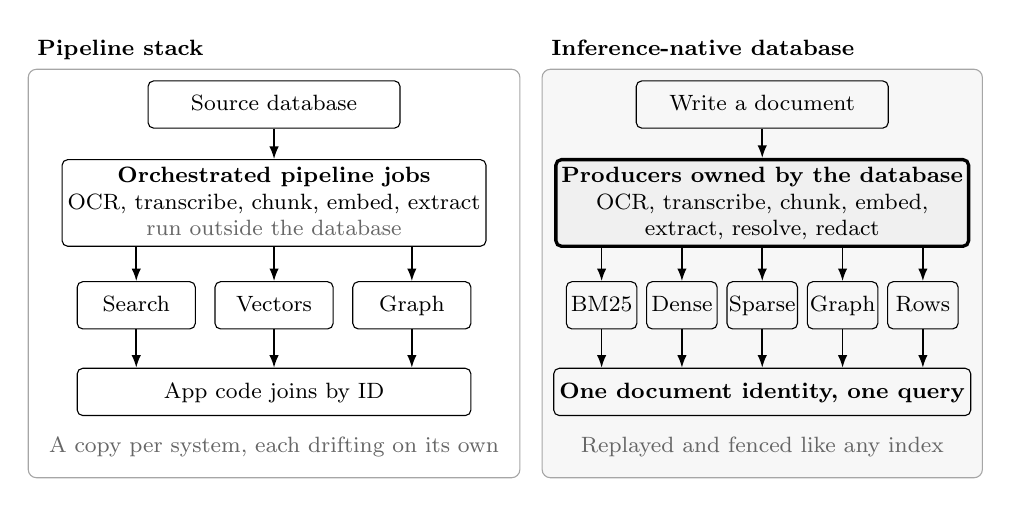
\begin{tikzpicture}[
    font=\footnotesize,
    box/.style={draw, rounded corners=2pt, align=center, inner sep=2pt,
                minimum height=6mm, text depth=.25ex},
    wide/.style={box, minimum width=50mm},
    mid/.style={box, minimum width=32mm},
    small/.style={box, minimum width=15mm},
    chip/.style={box, text width=8.6mm, inner xsep=0.5pt},
    accent/.style={very thick, fill=black!6},
    arrow/.style={-{Latex[length=1.6mm]}, semithick},
    note/.style={color=black!60},
    panel/.style={draw=black!35, rounded corners=3pt, inner sep=4pt},
    title/.style={font=\footnotesize\bfseries, anchor=south west, text depth=.25ex, text height=1.6ex},
  ]
  \def\rA{0}      % first box
  \def\rB{-1.25}  % producers / jobs
  \def\rC{-2.55}  % indexes
  \def\rD{-3.65}  % result
  \def\rE{-4.35}  % note

  % ---------------- Left: pipeline stack ----------------
  \begin{scope}
    \node[mid] (src) at (0,\rA) {Source database};
    \node[wide, minimum height=11mm] (jobs) at (0,\rB)
      {\textbf{Orchestrated pipeline jobs}\\OCR, transcribe, chunk, embed, extract\\{\color{black!60}run outside the database}};
    \node[small] (s1) at (-1.75,\rC) {Search};
    \node[small] (s2) at (0,\rC) {Vectors};
    \node[small] (s3) at (1.75,\rC) {Graph};
    \node[wide] (app) at (0,\rD) {App code joins by ID};
    \node[note] (lnote) at (0,\rE) {A copy per system, each drifting on its own};
    \draw[arrow] (src) -- (jobs);
    \foreach \s in {s1,s2,s3} {
      \draw[arrow] (jobs.south -| \s) -- (\s);
      \draw[arrow] (\s) -- (app.north -| \s);
    }
    \begin{scope}[on background layer]
      \node[panel, fit=(src)(jobs)(app)(lnote)] (lp) {};
    \end{scope}
    \node[title] at (lp.north west) {Pipeline stack};
  \end{scope}

  % ---------------- Right: inference-native database ----------------
  \begin{scope}[xshift=62mm]
    \node[mid] (w) at (0,\rA) {Write a document};
    \node[wide, accent, minimum height=11mm] (prod) at (0,\rB)
      {\textbf{Producers owned by the database}\\OCR, transcribe, chunk, embed,\\extract, resolve, redact};
    \node[chip] (c1) at (-2.04,\rC) {BM25};
    \node[chip] (c2) at (-1.02,\rC) {Dense};
    \node[chip] (c3) at (0,\rC)     {Sparse};
    \node[chip] (c4) at (1.02,\rC)  {Graph};
    \node[chip] (c5) at (2.04,\rC)  {Rows};
    \node[wide] (house) at (0,\rD) {\textbf{One document identity, one query}};
    \node[note] (rnote) at (0,\rE) {Replayed and fenced like any index};
    \draw[arrow] (w) -- (prod);
    \foreach \c in {c1,c2,c3,c4,c5} {
      \draw[arrow] (prod.south -| \c) -- (\c);
      \draw[arrow] (\c) -- (house.north -| \c);
    }
    \begin{scope}[on background layer]
      \node[panel, fill=black!3, fit=(w)(prod)(house)(rnote)] (rp) {};
    \end{scope}
    \node[title] at (rp.north west) {Inference-native database};
  \end{scope}
\end{tikzpicture}

  \caption{Left: every derived representation is a copy made by code outside
    the database. Right: the database owns the same work as index state,
    wherever the models run, and every index shares one document identity.}
  \label{fig:overview}
\end{figure*}

%--------------------------------------------------------------------------
\section{One identity across data models}
\label{sec:identity}

Multi-model databases place several engines behind one API. Antfly gives
every representation of a document one identity: source documents,
full-text indexes, dense and sparse vectors, graph relationships and
relational rows. A shared ID alone is not enough, since an external pipeline
can attach one too. Composition becomes reliable when shared identity comes
with a shared lifecycle: the same validity, publication, deletion and
permission rules govern every representation, so a set of documents means
the same thing in every index. We call this property \emph{polymorphism}:
one document, many representations. The sense differs from MongoDB's
polymorphic schema pattern~\cite{mongodb-polymorphic}, in which one
collection holds documents of many shapes.

A shared identity lets a query pass sets of documents from one index to
another instead of joining results in application code:
\begin{itemize}
  \item A structured or text filter narrows a vector search before ranking,
    not after.
  \item A graph traversal can start from the documents a hybrid search just
    ranked.
  \item An authorization rule is one more set of documents, applied by every
    retrieval operator.
\end{itemize}

Lifecycle ownership does not by itself produce composable data models, and
shared identity does not by itself make composition safe. Antfly makes both
choices. Ownership strengthens polymorphism, because every representation
inherits the same validity and permission rules; polymorphism amplifies
ownership, because one contract then covers every way a document is
retrieved.

%--------------------------------------------------------------------------
\section{What it enables}
\label{sec:enables}

Each capability in Table~\ref{tab:capabilities} is a separate product or
pipeline elsewhere. In Antfly each is a composition of the contracts in
\S\ref{sec:state} and \S\ref{sec:identity}, and each depends directly on
them. Further capabilities are listed in Appendix~\ref{app:capabilities}.

\begin{table}[t]
  \caption{Capabilities that depend directly on owning inference-derived
    state.}
  \label{tab:capabilities}
  \small
  \begin{tabularx}{\columnwidth}{@{}p{0.27\columnwidth}L@{}}
    \toprule
    Capability & What owning derived state makes possible \\
    \midrule
    Authorization inside retrieval & User and agent permissions apply inside vector search, text search, graph hops and agent tool calls. Filters take part in vector traversal instead of trimming results afterward, and model tool arguments cannot weaken them. \\
    Privacy across derived copies & Redaction is a rewrite of the producer graph, upstream of every chunk, embedding and text index, so no derived copy escapes it. \\
    Entity resolution & Extraction, matching and merging are replayed stages with recorded decisions and a canonical, editable entity table. \\
    Storage traded for inference & Vector indexes keep a fraction of each vector and recompute the rest on demand~\cite{wang2025leann}. This is safe only when source, model and revision are guaranteed together. \\
    \bottomrule
  \end{tabularx}
\end{table}

%--------------------------------------------------------------------------
\section{Related work}
\label{sec:related}

Several systems now manage some inference-derived state.
Elasticsearch chunks and embeds text at ingest~\cite{elastic-semantic-text},
and its preview \texttt{semantic} field also embeds images, audio, video and
PDFs~\cite{elastic-semantic}. Vespa runs models at feed time for embedding,
entity extraction, categorization, anonymization and
chunking~\cite{vespa-enrichment}. SurrealDB's Agent Memory, a closed-source
layer on its multi-model engine, extracts facts from documents with
provenance, temporal history and scoped grants~\cite{surrealdb-agent-memory}.

Existing systems manage important parts of inference-derived state. Antfly
makes the combined lifecycle contract (revision binding, recovery,
readiness and retrieval eligibility) an explicit database abstraction. We
therefore compare by property rather than by product category
(Table~\ref{tab:comparison}).

\begin{table*}[t]
  \caption{Comparison by property.}
  \label{tab:comparison}
  \small
  \begin{tabularx}{\textwidth}{@{}p{0.17\textwidth}LLLLL@{}}
    \toprule
    Property & Antfly & Elasticsearch & Vespa & SurrealDB & Postgres + extensions \\
    \midrule
    Inference managed at write time & Yes & Yes (embeddings) & Yes (embeddings and LLM enrichment) & In the Agent Memory layer & External worker \\
    Derived state beyond embeddings & OCR, transcription, extraction, resolution, redaction & Ingest processors for text extraction and entities & Extraction, anonymization, chunking & Fact extraction from documents & No \\
    Durable replay of derived state & Yes & Not documented & Not documented & Not documented & Not documented \\
    Model-revision binding & Enforced & Checks dimensions and similarity; same model advised, not enforced & Not documented & Not documented & Not documented \\
    Readiness semantics & Yes & Not documented & Not documented & Not documented & Not documented \\
    Shared identity across text, vector, graph, relational & Yes & Text and vector & Text and vector & Yes & Yes, across extensions \\
    Authorization inside retrieval & Yes & Document-level security in paid tiers & Application-level & Yes & Row-level security; applied after the vector index scan~\cite{pgvector,postgres-rls} \\
    \bottomrule
  \end{tabularx}
\end{table*}

Databricks offers the broadest platform, but its vector search indexes do not
inherit row- and column-level policies from source
tables~\cite{databricks-vector-search}.

The combination matters because the properties depend on each other:
readiness means little without revision binding, and retrieval eligibility
is unsafe without both. The closest precedent in form is the
lakehouse~\cite{armbrust2021lakehouse}, which argued that a second copy of
data was an artifact of system boundaries rather than a requirement. We make
the same argument about the copies created by inference pipelines.

%--------------------------------------------------------------------------
\section{Costs}
\label{sec:costs}

\begin{itemize}
  \item \textbf{Coupling.} Owning the lifecycle couples how an application's
    derivations evolve to database operations. Changing a producer graph
    behaves like a schema change: it starts a new generation, and an
    expensive graph, such as OCR over millions of pages or LLM extraction over
    a corpus, can take hours and real money to rebuild. Teams lose the
    freedom to ship a pipeline change on its own release cycle.
  \item \textbf{Where pipelines remain preferable.} Offline batch
    transformations with no serving path, models neither the runtime nor a
    provider can host, and derivations that join data living in several
    systems are better served by an external pipeline. Such a pipeline can
    still publish through the database's contracts.
  \item \textbf{Disaggregation.} Owning derived state does not require
    co-locating compute. Inference can run in a worker or a remote service;
    what moves into the database is the lifecycle, not the GPU. Independent
    scaling and fault isolation, the real strengths of pipelines, survive the
    move.
  \item \textbf{Availability versus safety.} Protected tables fail closed
    while privacy backfills run.
  \item \textbf{Combining permissions.} Antfly combines a user's role filters
    conjunctively, which is stricter than the permissive policies many
    database users expect. For agents, the stricter default is the right one.
  \item \textbf{Scope.} A larger engine has a larger failure surface, and a
    curated runtime runs fewer models than a general serving stack. Breadth
    comes from integrations instead: hosted model providers are first-class
    producers, with the same replay, readiness and permission semantics as
    local models.
\end{itemize}

\paragraph{Implementation.} Antfly is open source under Apache-2.0. It runs
as an embedded single file, a replicated server or a sharded cluster.

%--------------------------------------------------------------------------
\section{Evaluation}
\label{sec:eval}

\paragraph{Baselines.} Each experiment has a frozen, reproducible protocol in
the artifact repository~\cite{antfly-paper-repo}. The authorization
experiment compares PostgreSQL with pgvector (shared and partial HNSW indexes
under row-level security), ParadeDB native vectors, and LanceDB embedded with
prefiltering. The head-to-head compares against an external pipeline built to
succeed: Postgres with pgvector and row-level security, plus a durable
workflow engine such as Dagster or Temporal with lineage, versioned artifacts
and publication conditioned on the source version. Databricks serves as a
platform comparison.

Table~\ref{tab:experiments} lists five primary experiments, in priority
order, each with the result the design predicts.

\begin{table*}[t]
  \caption{Primary experiments.}
  \label{tab:experiments}
  \small
  \begin{tabularx}{\textwidth}{@{}p{0.16\textwidth}LL@{}}
    \toprule
    Experiment & Method & Predicted result \\
    \midrule
    Revision fencing & Swap the embedding model A $\rightarrow$ B $\rightarrow$ A during ingestion while querying continuously. & Zero queries observe a mixed vector space. \\
    Authorization under selective filters & On a public 1M-vector, 768-dimension corpus, vary permission eligibility from 50\% to 0.1\% of rows, random and correlated. Compare p50 and p95 latency at matched quality (recall@10 of at least 0.95 with ten authorized results), with Antfly at its default search effort and a top-10 post-filter ablation. & Antfly meets matched quality at every eligibility level without tuning; the post-filter ablation starves as filters tighten. \\
    Crash and update correctness & Crash after each producer stage; update and delete sources while enrichment is in flight. & No artifact from an obsolete generation becomes queryable. \\
    Privacy coverage & Plant personal data and inventory every stored artifact and external model request. & No protected derived representation contains an original value. \\
    Head-to-head on representative applications & Build call and meeting search with speaker turns, scanned-document search with OCR fallback and redaction, and permission-scoped agent retrieval over an extracted knowledge graph on Antfly and on the external pipeline. Drive each through the events in Table~\ref{tab:invariants}. & Both can maintain the invariants. We measure the coordination code, operating effort, recovery work and interference each needs, and report where ownership costs more, such as rebuild time and upgrade coupling. \\
    \bottomrule
  \end{tabularx}
\end{table*}

Secondary experiments measure throughput and GPU memory for a mixed workload
of PDFs, calls and video against separate services that each load their own
models; query latency while inference backfills; and storage and latency
when vectors are recomputed on demand. Reference implementations, counting
rules and workloads are published with the paper; generated code is excluded
from line counts.

%--------------------------------------------------------------------------
\section{Future directions}
\label{sec:future}

\begin{itemize}
  \item \textbf{Pipelines across documents.} Today a producer graph derives
    from one source document. The next step extends inference engineering
    across documents: dependencies on other documents, query results and
    complete graph selections, with freshness and lineage in both
    directions; integrity constraints on generated relationships; releases
    that switch sources and derived outputs to production atomically; and
    changefeeds that separate commits, published artifacts and release
    activations.
  \item \textbf{Redaction before storage.} Model-gated writes already exist
    (\S\ref{sec:state}). Running the privacy model inside them would keep
    original personal data from ever being stored.
  \item \textbf{Memory in latent space.} Memory modules that project stored
    embeddings into a frozen model's input space~\cite{fallahpour2026memorilla}
    need embeddings that are current, authorized and from one encoder
    revision, which are already database guarantees here.
  \item \textbf{Scheduling every resource.} Memory is unified under one
    manager today; GPU memory and time-sharing of GPU, CPU and disk between
    inference and storage maintenance come next.
  \item \textbf{A database that learns.} Antfly already learns its knowledge
    through entity resolution, memory and evaluation judges, and ships
    training kernels in the same runtime. Connecting them would train models
    from the database's own records and adopt each as a new revision through
    the existing generation switch.
\end{itemize}

%--------------------------------------------------------------------------
\section{Conclusion}

Inference-derived data should not be ordinary application-managed output.
Its validity depends on source versions, model revisions, readiness and
permissions, and those conditions must be enforced at the database's commit
and query boundaries, wherever the models run. Antfly makes that contract
explicit and reusable: replay, revision consistency, readiness,
authorization and privacy become database properties rather than pipeline
conventions. Every earlier workload brought its own index. Inference is the
next index builder, and the database should own its contract.

\bibliographystyle{ACM-Reference-Format}
\bibliography{references}

\appendix
\section{Additional capabilities}
\label{app:capabilities}

\begin{table}[h]
  \caption{Further capabilities built on the same contracts.}
  \label{tab:more-capabilities}
  \small
  \begin{tabularx}{\columnwidth}{@{}p{0.25\columnwidth}L@{}}
    \toprule
    Capability & What owning derived state makes possible \\
    \midrule
    Agent memory & Time-aware facts with evidence are stored in tables and indexes the database already maintains. \\
    Model-aware media & Chunk boundaries follow the consuming model's limits and the media's structure, such as speaker turns, pages and frames. \\
    Media planning & One pass over a recording or video feeds transcription, speaker detection and embeddings, and OCR runs only on pages whose native text fails a quality check. \\
    Resource scheduling & Model weights, inference caches, storage memtables, caches, compaction and indexes share one memory budget. Loading a model reclaims caches or defers optional compaction, and interactive work outranks background work. \\
    Models in queries & Typed model calls (\texttt{ai\_decide}, \texttt{ai\_choice}, \texttt{ai\_score}, \texttt{ai\_probability}) are operators in SQL and JSON queries. They run after authorization in a bounded stage and can be materialized as versioned write-time decisions. \\
    \bottomrule
  \end{tabularx}
\end{table}

\end{document}
